%%% Frontiers in Artificial Intelligence — Original Research
%%% "Disclosed Intelligence: A Large-Sample Measurement of AI Disclosure in U.S. Investment Adviser Fiduciary Filings"
%%% Compile: pdflatex -> bibtex -> pdflatex -> pdflatex

\documentclass[utf8]{FrontiersinHarvard}
\usepackage{url,hyperref,lineno,microtype,subcaption}
\usepackage{booktabs}
\usepackage{array}
\usepackage{calc}
\usepackage{longtable}
\usepackage[singlespacing]{setspace}
\linenumbers
\raggedbottom

\def\keyFont{\fontsize{8}{11}\helveticabold }
\def\firstAuthorLast{Chincholikar {and} Chawla}
\def\Authors{Samir Chincholikar\,$^{1}$, Robin Chawla\,$^{2,*}$}
\def\Address{$^{1}$Independent Researcher, New York, NY, United States \\ $^{2}$Independent Researcher, New York, NY, United States}
\def\corrAuthor{Robin Chawla}
\def\corrEmail{robin.chawla.cse14@iitbhu.ac.in}

\begin{document}
\onecolumn
\firstpage{1}

\title[Disclosed Intelligence]{Disclosed Intelligence: A Large-Sample Measurement of AI Disclosure in U.S. Investment Adviser Fiduciary Filings}

\author[\firstAuthorLast ]{\Authors}
\address{}
\correspondance{}
\extraAuth{}

\maketitle

\begin{abstract}
\section{}
Industry surveys suggest that registered investment advisers (RIAs) are increasingly using artificial intelligence (AI), but little is known about what advisers are disclosing to clients about AI in the fiduciary documents they provide. This study measures AI disclosure in a large sample of U.S. Form ADV Part 2A brochures, and explores variation in disclosure across adviser characteristics and between fiduciary filings and public marketing. We used the SEC Form ADV Part 1 population frame to identify 16{,}223 active SEC-registered advisers reporting regulatory assets under management and drew a stratified random sample of 400 firms by adviser type and AUM quartile. We classified existing brochures for 388 firms using a pre-specified five-label typology covering AI in investment processes, operations and client service, risk disclosure, explicit non-use, and named AI vendors or products. Classification was performed using a frozen large-language-model rubric, evaluated for same-family reproducibility, and independently validated through blinded cross-family recoding of 180 brochures. Disclosed AI use was 23.7\% of brochures (95\% CI 19.7--28.2) and was significantly associated with adviser size; private-fund advisers disclosed AI more often than wealth and retail advisers. The survey-weighted estimate for advisers who filed brochures was 22.7\% (95\% CI 18.7--26.6). The most common AI-related disclosure mode was risk disclosure, accounting for 27.6\%, which exceeded explicit claims of AI use. The main any-use measure demonstrated strong cross-family agreement ($\kappa = 0.74$; recall $= 0.84$; precision $= 0.76$). Language resembling the conduct described in SEC AI-washing enforcement actions was rare. Five brochures triggered the screening rule, and no brochures were identified as containing an unsubstantiated promotional claim. Among the 283 firms that were observed in both venues, 23.0\% disclosed AI use in fiduciary brochures versus 5.7\% on current websites. These findings indicate that disclosure of AI in adviser fiduciary filings is limited, is highly correlated with adviser size and type, and is substantively different from survey-reported adoption. Because survey-reported use and fiduciary disclosure are different constructs and different populations, it is appropriate to interpret their divergence as a contextual benchmark rather than a nondisclosure rate.

\tiny
 \keyFont{ \section{Keywords:} artificial intelligence, generative AI, investment advisers, Form ADV, fiduciary disclosure, text classification, large language models, AI-washing}

 \keyFont{ \section{Word count:} $\approx$9{,}600 (main text, per Frontiers' definition); Figures: 4; Tables: 6 }
\end{abstract}

\section{Introduction}

Artificial intelligence (AI) has quickly transitioned from experimental technology to operational capability claimed across financial services. Industry surveys suggest significant adoption among registered investment advisers (RIAs), with the Charles Schwab 2026 RIA and AI research study \citep{schwab2026} finding that about 63\% of surveyed firms are using or piloting AI. Such surveys give important insight into reported adoption, but they do not show what advisers disclose in the regulatory documents given to clients. Form ADV Part 2A, or the brochure, is a core narrative disclosure document for SEC-registered investment advisers that describes the adviser's business practices, investment strategies, conflicts, and material risks \citep{usSEC2019}. There is increasing interest in deploying AI in financial services, but there has not been an industry-scale measurement of the prevalence and format of AI disclosures in these fiduciary filings.

Measurement of such disclosure is important for regulatory and empirical reasons. Artificial intelligence can enter an advisory business through investment research, portfolio construction, trading, risk management, client service, operational processes, or third-party technology, and these uses may raise different disclosure considerations. Regulators have also started looking into whether firms accurately represent their AI capabilities. In March 2024, the U.S. Securities and Exchange Commission filed its first two enforcement actions related to misleading statements about the use of AI against Delphia and Global Predictions \citep{usSEC2024a,usSEC2024b}. The concern is similar to greenwashing, where claimed environmental credentials may be overstated compared to substantiated practices \citep{delmas2011,lyon2015}. But in the AI context the empirical problem is more than just spotting potentially exaggerated claims. A necessary first step is to develop a reproducible way to ascertain if companies mention AI at all, what type of use they disclose, whether AI is portrayed as a capability or a risk, and how such disclosure varies across firms.

This study thus takes a measurement-first approach to AI disclosure among U.S. investment advisers. We consider three substantive research questions. First, what is the prevalence of disclosed AI use in Form ADV Part 2A brochures and how does prevalence vary by adviser size and type? Second, when advisers talk about AI, is it more likely to be framed as a technology they use or a source of risk? Third, how do AI disclosures in the fiduciary brochure compare to the firms' public-facing marketing, and how often do either venue contain language similar to the types of AI claims identified in SEC enforcement actions? All three questions build on a methodological aim: to investigate if a large language model can serve as a reproducible measurement instrument for AI-related regulatory text if its classifications are compared to an independent blinded re-coding from a different model family.

We build the study from the structured data in the SEC Form ADV Part 1, identifying 16{,}223 active SEC-registered advisers reporting regulatory assets under management, and drawing a stratified random sample of 400 firms across adviser type and AUM quartile. We were successful in categorizing the current Form ADV Part 2A brochures for 388 firms. We employ a prespecified five-label typology that differentiates between AI use in investment process, AI use in operations or client service, AI-related risk disclosures, explicit statements of non-use, and references to named AI vendors or products. The classification rubric and model specification were specified before outcome analysis. We evaluate reproducibility within the same family and then perform a blinded, independent cross-family re-coding of 180 brochures, with validation statistics adjusted for the verification design. This enables the study to consider LLM classification not as an assumed source of ground truth but as a measurement procedure that can be explicitly assessed for its reliability and limitations.

The three main empirical results are as follows. First, 23.7\% of classified brochures report some form of AI use (95\% CI 19.7--28.2), with disclosure strongly increasing across adviser-size quartiles and more common among private-fund advisers than wealth and retail advisers. The size trend and adviser-type association are also robust to regression analysis ($p < 0.001$). The survey-weighted estimate for the brochure-filing population is comparable at 22.7\% (95\% CI 18.7--26.6). Second, AI is more frequently mentioned as a risk than as a claimed capability, with 27.6\% of brochures including an AI-related risk disclosure. Third, language similar to the conduct described in the two SEC AI-washing enforcement actions is not widespread. The enforcement-anchored screening rule triggered on five (1.3\%) of the classified brochures. Individual adjudication revealed that none involved unsubstantiated promotional claims of the kind charged in those actions. For the matched sample of 283 firms with both brochure and current website observations, disclosed use of AI is also much more likely to be found in brochures than in public-facing marketing, at 23.0\% and 5.7\%, respectively.

The difference between disclosed AI use observed in our sample and the roughly 63\% adoption found in the industry survey provides useful context but does not reveal a nondisclosure rate. The two measures differ in populations, dates, reporting settings, and constructs. Survey respondents may include experimental, administrative, or internal applications as AI use even where those applications are not material to a client-facing regulatory disclosure. Brochure language may describe algorithmic practices that respondents would not themselves describe as AI. Thus, for purposes of this study, the roughly 39-percentage-point gap is taken as a benchmark divergence between reported adoption and observed fiduciary disclosure, not as evidence that a corresponding proportion of advisers have adopted AI but have not disclosed it. To measure a real within-firm uptake-disclosure gap, information matching the AI usage of the sampled advisers would be necessary.

This study makes four contributions. First, it develops a predetermined and reproducible typology to measure AI-related disclosure in investment adviser filings and evaluates the resultant classifications by both same-family reproducibility and independent cross-family validation. Thus, the study contributes to the growing use of large language models as text-annotation tools by explicitly including validation, model dependence, and reproducibility in the research design \citep{gilardi2023,tornberg2023,ziems2024,rathje2024,ollion2024}. Second, it produces a large-sample estimate of disclosed AI use by SEC-registered investment advisers and documents systematic variation by adviser size and type using stratified sampling, uncertainty estimates, and population weighting. Third, it creates an enforcement-based filter for language similar to AI claims the SEC has charged before, and evaluates each positive case on its own, rather than assuming textual similarity equals misconduct. Fourth, it compares AI disclosure across regulatory and marketing venues and provides a reproducibility artifact that contains the frozen sample, classification rubric, prompts, validation materials, and analysis code. More generally, the paper extends the established use of financial and regulatory text as a firm-level measurement tool \citep{tetlock2007,loughran2011,hoberg2016,cohenLazy2020,abis2022} to an emerging and policy-relevant dimension of investment-adviser disclosure.

\section{Institutional background and related work}

\subsection{Form ADV and the fiduciary brochure}

Registered investment advisers with the SEC provide information about their business on Form ADV. Part 1 includes structured, machine-readable information about adviser characteristics, including legal identity, regulatory assets under management (AUM), client composition, private fund activities, and disciplinary history, and is made available through the SEC's public data infrastructure. Part 2A is the adviser's narrative brochure and describes matters such as advisory services, investment strategies, fees, conflicts of interest, and material risks, subject to applicable filing requirements and exemptions. Part 2A is different from Part 1, which mainly provides standardized firm-level variables, in that it provides narrative descriptions of how an adviser describes its practices and risks to clients.

This distinction makes the brochure a fitting setting for studying disclosed AI use. Advisory firms may engage in AI-related activity through investment research, portfolio construction, trading, risk management, client communications, operational processes, or third-party technology. Not all internal or experimental use of AI needs to be talked about in a regulatory brochure, and so the absence of AI terminology cannot be interpreted as evidence that a firm does not use AI. In contrast, to the extent an adviser explicitly discusses AI-related capabilities, processes, vendors, or risks in its brochure, that language constitutes an observable record of how the firm discusses AI in a formal disclosure context. Thus the object of this study is disclosure, rather than the underlying technology adoption. What we measure is what is written in the advisers' brochures, not whether a particular technology is actually deployed inside the firm.

\subsection{Enforcement of AI-washing}

In March 2024, regulatory scrutiny of AI-related disclosures intensified when the SEC announced settled enforcement actions against two investment advisers for making false or misleading statements about their purported use of AI. The SEC order alleges that Delphia (USA) Inc. did not develop the capabilities it claimed to have developed to use machine learning to analyze aggregate client data in a predictive algorithmic model. Global Predictions Inc. represented itself as the ``first regulated AI financial advisor'' and promoted ``AI-driven forecasts'' that the SEC found were not substantiated as advertised. The two companies agreed to civil penalties of US\$225{,}000 and US\$175{,}000, respectively \citep{usSEC2024a,usSEC2024b}.

These actions are relevant in a specific and limited way to the current study. They show that when firms make claims about AI capabilities that are false, misleading, or not sufficiently substantiated, this can become an enforcement problem. They also give two observable examples of the language of charged conduct. We thus use the orders to build an enforcement-based textual screen for potentially similar language in adviser disclosures and marketing materials. The screen is not designed to determine whether a firm has violated securities laws, and textual similarity alone is not evidence of misconduct. Instead, it raises a flag to check the document, and every positive case is assessed on its own merits against the underlying text. In the analysis, we call this kind of language potential AI-washing exposure language and not violations or proven cases of AI-washing.

\subsection{Related work}

The paper connects three research streams: textual measurement, large language models as annotation tools, and the economics of AI adoption and corporate disclosure. The first treats corporate and regulatory text as data from which firm characteristics that are otherwise hard to observe can be measured. \citet{tetlock2007} shows that textual information can contain economically meaningful signals, and \citet{loughran2011,loughran2016} show that financial language needs domain-specific measurement, as general-purpose linguistic categories can misclassify routine terminology in corporate disclosures. Related work uses filing text to construct measures of product-market similarity and competitive structure \citep{hoberg2016} and finds that changes in disclosure language contain economically relevant information \citep{cohenLazy2020}. Similar to the current design, \citet{abis2022} uses language from the prospectus to differentiate between quantitative and discretionary investment management and connects the text classification with observable fund behavior. More generally, \citet{grimmer2013} and \citet{gentzkow2019} highlight that text-based measures need to be evaluated as measurement tools, not as self-validated outcomes. This study applies that approach to AI disclosure in investment-adviser brochures and centers explicit validation in the research design.

A second body of literature examines whether large language models can reliably execute classification and annotation tasks that have historically been performed by human coders. Prior work demonstrates strong performance across a variety of social-science annotation settings, such as comparisons with crowd workers, zero-shot classification, multilingual measurement, and other computational social-science applications \citep{gilardi2023,tornberg2023,ziems2024,rathje2024}. At the same time, there are methodological concerns about using proprietary and ever-changing models. Model outputs can vary by version, prompt, and model family, and high apparent agreement does not guarantee a classifier has captured the intended construct \citep{bommasani2021,ollion2024}. Such concerns are especially salient when the outputs of LLMs become variables for substantive inference rather than simply tools for exploratory analysis. Thus, from the perspective of the LLM as a measurement instrument, its performance must therefore be evaluated. The classification rubric is prespecified, the primary model and snapshot are fixed, same-family reproducibility is reported separately, and a substantial subset of documents is independently re-coded by a different model family under blinded conditions. This design separates repeatability within a model family from agreement with an independent classifier.

The third strand concerns AI adoption, disclosure incentives, and potentially exaggerated technological claims. There is a growing literature on the economic implications of AI and related predictive technologies for labor demand, productivity, innovation, firm growth, and financial decisions \citep{agrawal2018,dacunto2019,acemoglu2022,eisfeldt2023,noy2023,babina2024,brynjolfsson2025}. Importantly, technological adoption is difficult to observe directly in itself. For instance, \citet{babina2024} derive firm-level AI investment from labor market information. Our setting poses a related, but different, measurement problem. The outcome of interest is not whether a firm has adopted AI, but whether it discloses AI-related activity in a fiduciary filing. The difference is important, because real adoption, self-reported adoption, and formal disclosure need not be the same.

Research on disclosure offers a framework for understanding why such differences may exist. Incentives for firms shape what information to disclose, how specific to be, and when proprietary, reputational, or regulatory concerns impact communication \citep{verrecchia2001,healy2001,leuz2016,blankespoor2020}. More recent work considers strategic disclosure also in settings where increasingly machines are processing corporate filings \citep{cao2024}. The possibility that claimed technological capabilities exceed substantiated capabilities is consistent with the established literature on greenwashing, where organizations can benefit from favorable claims while facing imperfect verification \citep{delmas2011,lyon2015}. This concern has direct relevance to investment advisers in light of the SEC's AI-related enforcement actions in 2024.

Taken together, the literatures motivate a measurement-centric approach that separates three concepts that could otherwise be conflated: underlying AI adoption, disclosed AI use, and potentially unsubstantiated AI claims. The latter two are considered in the present study as observable properties of regulatory and marketing text. It does this by applying a pre-specified classification framework to a large, stratified sample of adviser brochures, independently assessing the reliability of the resulting LLM-based measures, and using enforcement-derived language only as a screening mechanism that requires case-level adjudication. This approach offers an empirical baseline for researching AI disclosure, rather than assuming that no disclosure implies no adoption or that promotional language signals misconduct.

\section{Materials and methods}

\subsection{Population frame and sampling design}

The sampling frame was built from the SEC's Form ADV Part 1 bulk filing data. We merged 27{,}679 unique Central Registration Depository (CRD) identifiers that appeared in filings from 2011 to 2024 and kept advisers that were active as of December 31, 2024. Of the 16{,}709 active SEC-registered investment advisers, 16{,}223 reported regulatory assets under management (AUM) and were used as the population frame for sampling.

We used a stratified random-sampling design to ensure sufficient representation across adviser business model and firm size. Advisers were divided into two broad categories, private-fund advisers and wealth/retail advisers; and within each category, firms were assigned to AUM quartiles. The two adviser categories were crossed with four AUM quartiles to produce eight sampling strata. We then selected 50 advisers from each stratum using a fixed random seed, yielding an initial sample of 400 firms. The sample was drawn and frozen before retrieval or review of any Form ADV Part 2A brochure.

We decided to allocate evenly across the eight strata to ensure sufficient observations to compare across adviser types and across the AUM distribution. Given the deliberate oversampling of strata with fewer firms, especially larger advisers, unweighted sample proportions are not treated as direct population estimates. We therefore report both design-sample estimates and survey-weighted estimates that reestablish the population distribution across the eight sampling strata.

Structured sampling variables were extracted from the year-end 2024 Part 1 population frame, and brochure retrieval, website observation, classification, and validation were performed in 2026. The temporal difference is an explicit feature and limitation of the research design. Therefore, the frozen 2024 sampling strata are defined by the adviser type and AUM variables, rather than contemporaneous measures of firm characteristics on the exact date on which the 2026 disclosures were observed. The design should therefore be interpreted as capturing current disclosure among a probability sample drawn from the year-end 2024 population of active SEC-registered advisers reporting assets under management.

The target sample size of 400 was chosen to strike a balance between the needs for document collection and validation, and precision. For proportions near 50\%, a sample of $\sim$400 produces confidence intervals of $\sim\pm$4 percentage points at the aggregate level. Within individual strata of about 50 observations, expected confidence intervals are wider, generally on the order of $\pm$9 to $\pm$12 percentage points depending on the observed prevalence. Thus, the stratum-level estimates are interpreted mainly for broad patterns, and formal tests of the size gradient are performed on the combined sample.

\subsection{Form ADV Part 2A collection and analysis sample}

For each sampled adviser, we attempted to obtain the current Form ADV Part 2A brochure filed with the SEC's public filing system. Of the 400 sampled firms, 388 produced a brochure with usable text for the primary classification analysis. Eleven companies were not required to file a Part 2A brochure under the relevant filing circumstances, while one additional brochure could not be converted into usable text. All 12 excluded observations were in the wealth/retail adviser category.

The main estimand is thus AI disclosure among advisers with an observable Form ADV Part 2A brochure, rather than among every adviser in the original Part 1 sampling frame. Firms that are exempt from filing brochures are not considered to have zero AI disclosure, since the lack of a required brochure is conceptually different from a brochure that does not mention AI. As a sensitivity analysis we also examined the effect of classifying unclassified observations as non-disclosers. This does not change the substantive conclusions and changes aggregate prevalence by no more than about three percentage points.

All retrieved source documents were stored with content hashes to keep the exact text analyzed. Document processing was finalized before substantive outcome analysis. The resulting analytical corpus consists of the 388 brochures that were successfully classified.

\subsection{Classification of AI disclosure}

We created and locked in a five-label classification framework to distinguish substantively different forms of AI-related disclosure prior to outcome analysis. The categories were designed to distinguish substantively different forms of AI disclosure.

The first category, \textbf{investment-process AI}, includes statements that refer to the use of AI, machine learning, or closely related computational methods in investment research, security selection, portfolio construction, trading, forecasting, or other elements of the investment process. The second category, \textbf{operations or client-service AI}, tracks the disclosed use of AI in functions such as client interaction, administrative processes, workflow automation, compliance, communications, or other non-investment activities. The third category, \textbf{AI risk factor}, captures language identifying AI or related technologies as a source of operational, investment, cybersecurity, model, regulatory, or other risk. The fourth category, \textbf{explicit non-use}, is made up of positive statements that the adviser does not use AI or does not use AI for a specified activity. The fifth category, \textbf{named vendor}, captures mentions of a specific vendor, platform, model, or product related to AI.

These labels were used to create two composite measures. \textbf{Any AI use} equals one when a brochure includes AI in investment process, operations/client service, or a named AI vendor or product. We also report any-use prevalence after excluding the vendor category, since a vendor reference may sometimes be a weaker signal of direct firm-level use than an explicit description of an AI-enabled activity. \textbf{Any AI mention} covers any of the five labels, including risk disclosures and explicit non-use.

For each positive classification, verbatim quotes from the brochure were needed to provide support. The classification rubric was frozen before the prevalence results were calculated and included inclusion and exclusion criteria and examples for each label. The reproducibility materials include the full rubric, the prompts, the text-window specification, the model snapshot, and the classification date.

\subsection{Primary LLM classification}

The 388 brochures were classified using GPT-4o as the main large language model. To minimize avoidable generation variability, a fixed model snapshot was used with the temperature set to zero. Each brochure was scored using the prespecified rubric, and the model was required to output the relevant binary labels along with supporting text for positive classifications.

The LLM was used as a measurement instrument, not as an assumed ground truth. The study therefore distinguishes primary classification from reliability and validation exercises that follow. This distinction is important because deterministic settings can enhance repeatability without establishing construct validity, and agreement between repeated outputs from the same model family does not provide the same evidence as agreement with an independently generated classification.

To assess within-family reproducibility, 60 brochures were randomly selected and independently reclassified by GPT-4o-mini using the same frozen rubric. Agreement was calculated for each label and also for the composite any-use measure. These statistics are used as measures of same-family reproducibility, not external validation.

\subsection{Independent validation across families}

A separate validation exercise was performed using an independently operated model by another provider and model family: a total of 180 brochures were re-coded with Anthropic Claude using the same frozen definitions but without access to the GPT-4o classifications. Thus, this re-coding was blind to the primary labels.

The validation sample was intentionally oversampled for primary-model positives to ensure sufficient observations to estimate classification performance. We included all 123 brochures that the primary model classified as positive for the composite any-use measure, and a fixed-seed random sample of 57 brochures chosen from the 265 primary-model negatives. So, na\"ive validation statistics would not reproduce the distribution of the full analytic sample, because primary positives and negatives had different probabilities of entering the verification sample.

We therefore used inverse-probability verification weights in estimating metrics influenced by the sampling design. Weighted recall, agreement, and Cohen's $\kappa$ \citep{cohen1960} were calculated to represent the full classified sample. Verification weighting does not impact the precision of the any-use measure, because all primary-model positive cases were included in the validation set. We also report per-label agreement statistics and F1 scores.

Cross-family re-coding presents a more difficult test than same-family replication, as it reduces dependency on a single model architecture and provider. This is still model-to-model validation, not expert human adjudication. We do not claim the independent re-coding to be the ultimate ground truth. Residual disagreement is left as a defined set for subsequent human expert review, and this limitation is explicitly considered in the interpretation of the results.

\subsection{Enforcement-anchored exposure-language screen}

To determine whether adviser communications contain language similar to the disclosures that the SEC has previously found in enforcement actions, we developed a narrow screening method based solely on SEC orders concerning Delphia (USA) Inc. and Global Predictions Inc. Seven textual claim patterns were distilled from the representations cited in those two actions and applied to the brochure corpus.

This procedure was intentionally designed as a high-sensitivity screen and not as a legal classifier. A document was flagged if its language was sufficiently similar to one or more of the enforcement-derived claim patterns as to require manual review. Thus, a positive screen is only potential exposure language and is not evidence of false statements, inadequate substantiation, or a securities-law violation.

The number of flagged documents was small, and each positive case was evaluated in relation to its surrounding text. The cases were then categorized according to whether the language was a false-positive textual match, an AI-related statement with supporting context or risk disclosure, or a potentially unsubstantiated promotional claim similar to the conduct described in the two enforcement orders. Results are reported in aggregate form, without identifying individual advisers.

\subsection{Website collection and cross-venue comparison}

We generated a matched website sample for the sampled advisers to compare fiduciary disclosure with public-facing communication. Firm websites were collected using a standardized retrieval protocol on the homepage and on the main pages describing the firm, its investment approach, services, or technology. We collected up to eight pages per firm with the request rate limited to about one per second. Classification was made on the basis of the principal text rendered available from these pages.

Usable website observations were obtained for 283 of the 400 advisers sampled. The resulting analysis is therefore a matched cross-venue comparison, rather than a full census of the original sample. To determine whether website availability was systematically associated with observed adviser characteristics, we compared firms with usable website data to firms without such data by adviser type, AUM quartile, and AUM level.

The website measure only captures the current principal web presence of the firm at the time of collection. It is not a comprehensive coverage of dynamically rendered content that could not be retrieved, archived website versions, press releases, social media accounts, third-party profiles, or other marketing channels. Thus, the analysis is a comparison of current Form ADV Part 2A disclosure and current principal-site marketing, rather than regulatory disclosure and the full universe of the firm's communications.

\subsection{Statistical analysis}

For each classification label and composite measure, we report the observed prevalence and 95\% confidence intervals. For unweighted binary proportions we use Wilson intervals \citep{wilson1927}, which have better finite-sample coverage than the normal approximation, especially when the prevalence is somewhat low or when the estimates are calculated within smaller strata.

Ordered trend tests are used to test for differences by adviser size, with AUM quartile as an ordinal variable. We also estimate a logistic regression with disclosed any-use as the dependent variable and AUM quartile and adviser type as the main predictors. The regression is meant to assess whether the size gradient holds after controlling for the broad private-fund versus wealth/retail distinction; it is not interpreted causally.

Because the equal-allocation sampling design does not reflect the population distribution of the eight sampling strata, a survey-weighted estimate is also calculated. Stratum weights are calculated from the population counts in the 16{,}223-adviser Part 1 frame and adjusted to reflect the brochure-filing population using the observed filing rate within each stratum. The variance of the stratified design provides an estimate of the associated uncertainty. As a further check on sensitivity, we compute an unadjusted population-weighted estimate for the entire 16{,}223-firm frame. This enables us to assess the practical effects of brochure-filing exemptions on the aggregate estimate.

For the matched brochure-website sample, we compute within-firm differences in prevalence across the two venues. We calculate the uncertainty of the venue difference by a paired bootstrap that samples firms, not individual documents, so as to maintain the matched structure of the observations.

All tests are two-tailed. We apply conventional cutoffs to evaluate statistical significance, but the substantive interpretation focuses on effect size, confidence intervals, and robustness across sensitivity analyses rather than significance as such.

\subsection{Robustness and reproducibility}

The empirical design includes a number of pre-specified or easily replicable checks. We re-estimate any-use prevalence excluding named-vendor references, estimate prevalence using independent cross-family classifications, assess alternative treatment of brochures unavailable for classification, compare design-sample and population-weighted estimates, report same-family and cross-family agreement separately, adjudicate every enforcement-screen positive individually, and re-estimate the principal adviser-type pattern using the independent coder.

Before assessing substantive results, the sampling, classification framework, text-processing rules, prompts, model specification, and principal outcome definitions were frozen. The reproducibility package contains the frozen sample, the classification rubric, the prompts and text-window specification, the model snapshot and classification date, the enforcement-screen fingerprint, the population stratum counts, the weighting and statistical-analysis code, the validation records, the independent cross-family classifications, and the scoring code. A deterministic executable environment is provided to allow the reproduction of the reported tables, figures, confidence intervals, weighted estimates, and validation statistics from the study.

Adviser identifiers are pseudonymized, and the mapping from adviser identifiers to CRD numbers is withheld; thus the public package supports analytical reproducibility rather than full reconstruction of the original raw-document collection. The underlying Form ADV data is publicly available from the SEC, but producing the exact source-document corpus would require access to the withheld identifier crosswalk.

\section{Results}

\subsection{AI disclosure: prevalence and form}

Of the 388 advisers with successfully classified Form ADV Part 2A brochures, 23.7\% disclosed at least one form of AI use (95\% CI 19.7--28.2; Table~\ref{tab:typology}, Figure~\ref{fig:typology}). Eliminating references to specific vendors from the composite definition modestly reduced the prevalence to 20.9\%, suggesting that the main estimate is not solely driven by mentions of third-party AI products. The wider any-mention measure, which captured disclosed use, AI-related risk language, explicit non-use, and vendor references, was 31.7\%.

Disclosures related to risks associated with AI occurred more often than affirmative disclosures about AI use. Overall, 27.6\% of the brochures had language that referenced AI, machine learning, or related technology as a source of investment, operational, cybersecurity, model, regulatory, or other risk. The pattern is that AI appears in investment-adviser brochures as a disclosed technological capability, but more often it is something to be warned about. The distinction is important because a risk-factor reference does not imply the adviser itself uses AI. Hence, risk disclosure is reported separately from the any-use measure across the analysis.

The survey-weighted estimate of the proportion of brochure-filing advisers that disclosed use of AI was 22.7\% (95\% CI 18.7--26.6; Table~\ref{tab:weighting}), very similar to the unweighted design-sample estimate of 23.7\%. Weighting straight to the full 16{,}223-adviser population frame, without adjustment for brochure-filing status, produced a similar estimate of 22.3\%. The small difference between these estimates implies that the prevalence rate is not greatly affected by either the equal-allocation stratified sampling design or the small number of brochure-filing exemptions.

\subsection{Disclosure by size and type of adviser}

The disclosed use of AI grew substantially with adviser size (Table~\ref{tab:gradient}, Figure~\ref{fig:gradient}). Among private-fund advisers, prevalence increased from 12\% in the lowest AUM quartile to 24\% in the second quartile, 34\% in the third quartile, and 56\% in the highest quartile. The corresponding estimates for wealth and retail advisers were 8.7\%, 8.3\%, 14.6\%, and 30.4\%. Hence, the pattern is not limited to one adviser category: both groups show much higher disclosure for larger firms, although the gradient is steeper for private-fund advisers.

These patterns were confirmed by ordered trend tests. For private-fund advisers, the linear-by-linear trend across AUM quartiles was strongly positive ($z = 4.82$, $p < 0.00001$). The trend was also significant for wealth and retail advisers ($z = 3.00$, $p = 0.003$) and the combined sample ($z = 5.57$, $p < 0.0000001$).

The same substantive conclusion was reached using a logistic regression with disclosed any-use as the dependent variable. AUM quartile was positively associated with AI disclosure after controlling for adviser type (coefficient $= 0.67$, SE $= 0.12$, $p < 0.001$), and private-fund advisers were more likely to disclose AI than wealth and retail advisers conditional on size quartile (coefficient $= 1.01$, SE $= 0.27$, $p < 0.001$). These coefficients are descriptive associations rather than causal estimates, but they show that the observed size gradient is not due merely to the different distribution of private-fund and wealth/retail advisers across the AUM strata.

\subsection{Classification reproducibility and independent validation}

The same-family reproducibility exercise showed broad agreement, but also suggested that some substantive categories were harder to classify consistently than others. Cohen's $\kappa$ was 0.95 for AI risk disclosure and 1.00 for named-vendor references. Agreement was also high for the broader any-mention measure ($\kappa = 0.86$). The $\kappa$ values for AI in investment processes and operations or client services were lower, at 0.61 and 0.66, respectively. Same-family agreement for the composite any-use measure was $\kappa = 0.69$.

The independent cross-family validation provided a more demanding test (Table~\ref{tab:validation}, Figure~\ref{fig:validation}). Taking the verification-sampling design into consideration, the composite any-use measure obtained a precision of 0.76, a recall of 0.84, an F1 score of 0.80, an overall agreement of 90.8\%, and a Cohen's $\kappa$ of 0.74. Hence, the main classifier identified most of the independently identified positive cases and showed substantial agreement with the blinded cross-family re-coding.

Performance varied by classification category. AI risk disclosure showed the strongest classification performance (precision 0.92, recall 0.99, F1 0.95, agreement 97.4\%, $\kappa = 0.93$). Operations or client-service AI yielded precision of 0.81, recall of 0.68, F1 of 0.74, agreement of 96.1\%, and $\kappa = 0.72$. Investment-process AI was more difficult to distinguish consistently (precision 0.69, recall 0.74, F1 0.71, agreement 89.8\%, $\kappa = 0.65$). Explicit non-use resulted in high overall agreement (97.7\%) and low $\kappa$ (0.60), as it was rare. Named-vendor references resulted in 97.4\% agreement and $\kappa = 0.68$.

Adjusted prevalence was about 21.6\% following re-estimation from the independent cross-family classifications for disclosed any-use. This estimate is within the confidence interval of the main 23.7\% estimate and maintains the main adviser-type pattern. Hence, the substantive prevalence finding is not contingent on the assumption of error-free primary LLM classifications.

\subsection{Enforcement-anchored exposure-language screen}

Of the 388 brochures in the classified sample, five (1.3\% of the classified sample; 95\% CI 0.6--3.0) were identified for case-level review using the enforcement-derived screen. The screen was designed to identify textual resemblance, not misconduct, so all five positive cases were examined individually in context.

Two were false-positive textual matches in which the relevant language did not constitute an affirmative promotional claim regarding the adviser's AI capabilities. The other three had actual references to AI or machine-learning activities, but also contained contextual or risk-related language that bolstered or qualified the statements. None was adjudicated as an unsubstantiated promotional claim of the nature alleged in the SEC's two enforcement actions.

The resulting estimate should not be taken as the prevalence of AI-washing. The screen captures only language that appears to be a narrow set of claim patterns that come from two enforcement cases, and the number of positives is small. Rather, the result suggests that language similar to the charged representations was rare in the sampled fiduciary brochures and that the screening procedure did not produce a single instance that could be classified as an unsubstantiated promotional claim based on the text available.

\subsection{Fiduciary disclosure and public-facing marketing}

Current website observations were obtained and usable for 283 sampled advisers. Within this matched sample, disclosed AI was found in 23.0\% of Form ADV Part 2A brochures, but only in 5.7\% of current principal-site marketing materials (Table~\ref{tab:venue}). The difference is substantial and does not support the interpretation that AI claims are largely confined to promotional material aimed at the public.

This pattern is supported by the underlying matched observations. Fifty-eight firms disclosed AI usage in their brochure but not on the observed website, with only nine disclosing the opposite pattern. Thus, among firms with both venues visible, disclosure in the brochure only was much more common than disclosure on the website only.

The enforcement-anchored exposure-language measure was rare in both venues: about 0.7\% of observations in each. The paired bootstrap estimate of the difference was essentially zero (95\% CI approximately $-0.014$ to $0.014$). There is no evidence in the matched sample, therefore, that the narrow enforcement-derived language patterns were more prevalent on current websites than in fiduciary brochures.

There was also little evidence of systematic selection on observed sampling characteristics in website availability (Table~\ref{tab:missingness}). Coverage did not differ significantly by adviser type ($p = 0.83$) or AUM quartile ($p = 0.50$). The median AUM for firms with usable website observations was approximately US\$419 million and US\$357 million for those without, a difference that was not statistically significant ($p = 0.46$). None of these comparisons establish that missingness of websites is random conditional on all unobserved characteristics, but they do alleviate concerns that the matched sample is mechanically concentrated among one of the principal adviser categories considered in the study.

\subsection{Robustness of the principal findings}

Key prevalence and cross-sectional findings are robust to alternative measurement and weighting options. Removing named-vendor references reduces disclosed any-use from 23.7\% to 20.9\%, but does not change the substantive conclusion. Re-estimation using the independent cross-family classifications yields a prevalence of about 21.6\%, also within the primary confidence interval. The alternative treatment of the 12 firms with no classified brochures changes the aggregate prevalence only modestly.

Weighting does not materially change the result either. The unweighted stratified-sample estimate is 23.7\%, the survey-weighted estimate for brochure-filing advisers is 22.7\%, and direct weighting to the original 16{,}223-adviser population frame yields 22.3\%. The close correspondence across the three estimates suggests that the aggregate finding is not an artifact of the equal-allocation sampling design.

The validation exercises also provide a consistent ordering of measurement reliability. More explicit constructs, particularly AI risk disclosure, had the highest agreement, whereas distinctions such as the precise functional use of AI were less reliable. Importantly for the central result, the any-use measure shows substantial agreement under independent cross-family validation, and the main prevalence and adviser-type results are not overturned by replacing the primary labels with the independent classifications.

Together, these checks indicate that the central conclusions do not depend on any single label definition, weighting scheme, missing-brochure handling, or LLM classification run. Roughly one-fifth to one-quarter of observed adviser brochures across specifications disclose some form of AI use. Disclosure increases significantly with adviser size. Private-fund advisers disclose AI more often than wealth and retail advisers. AI-related risk language is common relative to affirmative use claims. Current fiduciary brochures include significantly more disclosed AI use than the matched firms' principal websites.

\section{Discussion}

\subsection{Main findings}

This study provides large-sample evidence on U.S. investment advisers' artificial intelligence disclosures in Form ADV Part 2A brochures and how those disclosures vary across firms and communication venues. Three findings are especially important. First, disclosed AI use is still limited to a small subset of adviser brochures (23.7\% observed, 22.7\% survey-weighted among brochure-filing advisers). Second, disclosure is systematically different across the advisory industry, increasing sharply with adviser size and being more common among private-fund advisers than wealth and retail advisers. Third, AI is not only a claimed technological capability in fiduciary filings, but it is also a source of risk, with AI-related risk disclosure in 27.6\% of brochures.

The results provide an empirical baseline for disclosure of AI in the U.S. investment adviser industry. They also demonstrate why the disclosure of artificial intelligence cannot be simplified into a binary distinction between AI-using and non-AI-using firms. Advisers disclose AI in a number of ways---its application to investment activities, its use for operational or client-service functions, reliance on third-party products, and the risks of emerging technologies. The resulting disclosure landscape is therefore heterogeneous across firms and in the language firms use to describe AI.

\subsection{AI disclosure and reported industry adoption}

The extent to which companies are reporting the use of AI in regulatory filings is substantially below the levels of AI adoption reported in industry surveys. This is contrasted to survey evidence that some 63\% of advisers either use or are piloting AI, and to the roughly 23\% of brochures in the present study that disclose some form of AI use. This difference is economically meaningful as a benchmark, but should not be interpreted as a direct estimate of nondisclosure.

The two measures are tapping different constructs. Industry surveys tend to measure self-reported adoption, experimentation, or intended use among participating firms. The present study measures whether AI-related activity appears in a formal fiduciary document. An adviser may use AI for internal administrative purposes, exploratory applications, or other functions without determining that such use is sufficiently material to be included in its brochure. Conversely, a brochure could mention algorithmic processes, machine-learning methods, or third-party technologies that respondents might not classify as AI themselves in responding to a survey.

Other limitations to direct comparison include differences in sampling populations, observation dates, and reporting incentives. The approximately 39-percentage-point gap between the external survey benchmark and observed brochure disclosure should therefore be interpreted as a gap between self-reported adoption and formal disclosure---not as evidence that a similar share of advisers are using AI in practice without disclosure. To identify a real adoption-disclosure gap, we would need matched information on technological use and regulatory disclosure for the same firms at the same point in time.

This distinction is important because if one conflates adoption with disclosure, the findings could be interpreted in an overly strong regulatory way. The evidence here shows that formal disclosure of AI is far less prevalent than survey-reported AI use, but does not address whether undisclosed uses are immaterial, experimental, misreported in surveys, or otherwise outside the scope of brochure disclosure.

\subsection{Adviser size and differences in business models}

One of the most robust empirical patterns is the strong correlation between adviser size and AI disclosure. Among private-fund advisers, disclosed AI use increases from 12\% in the lowest quartile of AUM to 56\% in the highest quartile. Wealth and retail advisers have prevalence rates ranging from around 9\% in the lower quartiles to 30.4\% in the highest quartile. The positive size gradient remains statistically significant when adviser type is added to the regression model.

There are a few plausible mechanisms that might generate this relationship. Larger firms may be better placed to develop or acquire AI systems, as they have more financial, technical, and organizational resources. They may have more complex investment, risk-management, compliance, and client-service infrastructures, which generate a broader range of activities in which AI-related technologies can be incorporated. Larger organizations may also have increased compliance capacity and more formalized procedures for documenting emerging technologies in regulatory filings.

The current design does not disaggregate these mechanisms, and the observed association should not be taken as causal. There may be a relationship between adviser size and investment strategy, organizational sophistication, client composition, technology budgets, regulatory scrutiny, or other characteristics that independently affect disclosure. Still, the result shows AI disclosure is not evenly distributed across the adviser universe, and that firm size is strongly associated with whether AI is disclosed in fiduciary filings.

An additional aspect of heterogeneity concerns the adviser type. We find that private-fund advisers are more likely to disclose AI conditional on AUM quartile than wealth and retail advisers. Private-fund managers may be more likely to use systematic investment approaches, alternative data, quantitative research processes, or specialized technology infrastructure that generates disclosure-relevant references to machine learning and artificial intelligence. But the type of adviser also encompasses more general differences in investment strategy, client base, organizational structure, and disclosure practice. As such, the finding should be understood as a strong descriptive association, not as an indication that the private-fund business model per se causes greater AI adoption or disclosure.

\subsection{AI as a disclosed capability and a disclosed risk}

The findings also underscore a crucial difference between AI as a claimed capability and AI as a source of risk. 27.6\% of brochures contain AI-related risk language, a higher rate than the primary any-use measure. This finding suggests that simply including the term AI in a regulatory filing does not necessarily mean the adviser is using the technology.

Artificial intelligence, machine learning, generative AI, or other such technologies can be described in a brochure because those technologies generate cybersecurity, investment, operational, model, legal, or regulatory risks. Therefore, using any reference to AI as a proxy for adoption would overstate the extent of disclosed AI use. This is especially important for automated text analysis, where simple keyword-based measures may combine conceptually different statements into a common indicator.

This paper describes the five-label framework that addresses this problem by separating investment-process use, operations or client-service use, risk disclosure, explicit non-use, and named-vendor references. The difference between these categories is not only methodological. The findings suggest that advisers use AI in fiduciary disclosure across multiple communicative functions. Some advisers describe AI as a capability, whereas others discuss it primarily as a source of risk.

The high level of risk disclosure may also be a function of the broader role of Form ADV Part 2A as a fiduciary disclosure document. Brochures are designed, in part, to describe material practices, conflicts, and risks, as opposed to promotional communications. The prominent role of caution with regard to AI in this context is thus consistent with the institutional role of the document, although the cross-sectional design cannot establish the reasons why individual advisers opted for particular language.

\subsection{Enforcement-related language and cross-venue disclosure}

The enforcement-anchored analysis provides a complementary perspective on AI-related representations. The textual screen derived from the two SEC AI-related enforcement actions triggered on only five of the 388 brochures, none of which was adjudicated as containing an unsubstantiated promotional claim of the type described in those actions. Thus, close textual correspondence with the particular representations alleged in those cases was uncommon in the fiduciary filings in the sample.

Results should be interpreted with caution. The screening procedure depends on just two enforcement actions and is unable to capture all possible types of misleading AI representation. Access to internal systems, records, development histories, or other evidence not publicly filed may also be needed to determine whether a statement is false or not adequately substantiated, and no textual classifier can make such a legal or factual determination from language alone.

The contribution of the enforcement screen is thus methodological, not accusatory. Enforcement actions can be used to develop observable claim patterns that help identify documents for more detailed review, but screen positives need to be evaluated in context. Of the five flagged brochures in the current sample, two were false-positive textual matches and three had bona fide AI or machine-learning references with contextual or risk-related language. None provided sufficient textual evidence to classify the statement as an unsubstantiated promotional claim. The study therefore does not estimate a prevalence of AI-washing across the industry and does not take textual similarity as evidence of misconduct.

The cross-venue analysis further complicates an exclusively promotional interpretation of AI disclosure. We find AI use in 23.0\% of the 283 advisers with both a Form ADV brochure and a current principal website, and in 5.7\% of the 283 websites. Fifty-eight companies demonstrated AI usage in their brochure but not on their website, whereas only nine exhibited the reverse pattern.

If advisers had been using AI terminology largely as a marketing device, we might have expected to see more of it in public-facing website content. Instead, the results show significantly more AI disclosure in the fiduciary filing. One possibility is that Form ADV brochures contain more detailed descriptions of investment processes, operational practices, third-party technologies, and associated risks than companies choose to disclose on their main websites. Websites might instead focus more on investment philosophy, client relationships, services, or brand positioning.

This comparison is still limited by the website-collection procedure. The analysis covers current principal-site content and is not representative of all marketing communications. Social media, advertisements, press releases, archived pages, and inaccessible dynamically rendered material are not comprehensively included. Accordingly, the finding should be considered as evidence of a difference between current fiduciary brochures and current principal websites, rather than a complete comparison between regulatory disclosure and all forms of adviser marketing.

\subsection{Methodological implications of LLM-based regulatory measurement}

This paper also provides evidence on the use of large language models as a measurement instrument for regulatory text. Classification performance differed substantially among disclosure categories. The most robust independent agreement was produced by explicit AI risk language, with the line between investment-process use and operational use being more difficult to reliably classify. This variation demonstrates how conceptually ambiguous apparently straightforward text labels can be.

Nevertheless, independent cross-family validation of the primary any-use measure showed substantial agreement (Cohen's $\kappa = 0.74$; recall $= 0.84$; precision $= 0.76$; F1 score $= 0.80$). Re-estimating prevalence from the independent classifications produced a value of about 21.6\%, which lies within the confidence interval of the main estimate of 23.7\%. The main substantive conclusion, therefore, does not depend on perfect agreement between the two classifiers.

We distinguish between intra-family reproducibility and cross-family validation. Repeating the classification with models from the same family can show that the procedure is reasonably stable, but it does little to argue against a model-specific interpretation. A blinded classifier from a different provider or model family creates a more independent test, as validation labels are not created by the same model architecture, nor are they directly conditioned on the original outputs. The stronger agreement for some categories and weaker agreement for others also contains information that would be lost if validation were summarized by one overall accuracy statistic.

However, cross-family validation is not a definitive ground truth. Models might also share patterns in training data, conceptual biases, or problems understanding ambiguous regulatory language. Hence, human domain-expert adjudication remains an important extension, particularly for the residual disagreement set and the less reliable categories. The results support the use of LLMs to measure regulatory text at scale, provided that the classification procedure is explicitly validated rather than treating model output as inherently correct.

More broadly, the research design demonstrates how LLM-based classification can be used in empirical financial and regulatory research without obscuring the analytical process. The classification categories were defined before outcome analysis, the model configuration and rubric were fixed, each positive classification was text-supported, independent validation was conducted in a blinded manner, and the verification-sampling design was part of the reported performance metrics. The reproducibility materials also reproduce the output variables and statistical results from the published analytical data.

These procedures are especially important when LLM classifications are used as inputs for substantive statistical inference. In such settings, model output is not just an aid in reading documents, but part of the measurement process through which empirical claims are generated. Making the classifier explicitly a fallible measurement instrument makes uncertainty, disagreement, and reproducibility visible, not implicit. The results show that the proposed method can scale the analysis of large regulatory corpora while providing a clear basis for evaluating the generated measures.

\section{Limitations and future research}

\subsection{Limitations}

Several limitations qualify the interpretation of the findings. First, the study measures disclosed AI use, not underlying technology adoption. Form ADV Part 2A captures how advisers describe their practices and risks through a regulatory document, but does not provide direct observation of the technologies actually deployed within the firm. One adviser might use AI internally and not mention it in its brochure, while another might describe quantitative, algorithmic, or vendor-supported processes that are on the border of what should be classified as AI. The estimates should therefore be interpreted as measures of disclosure, rather than actual AI adoption.

Second, the disclosure observations are not contemporaneous with the sampling frame. Adviser type and AUM quartile were determined from the 2024 year-end population of Form ADV Part 1. Brochure retrieval, website collection, classification, and validation occurred in 2026. Thus the stratification variables describe firms at the time the probability sample was drawn, not their exact characteristics at the time the later disclosures were observed. In the meantime, firms may have altered their size, business model, registration status, or disclosure practices. Therefore, the results are best interpreted as 2026 disclosure outcomes for advisers sampled from the year-end 2024 population frame. The timing structure preserves the integrity of the frozen probability sample but limits claims about contemporaneous relationships between 2026 AUM and disclosure.

Third, the validation design relies on independent re-coding by LLMs, rather than expert human annotation. The blinded cross-family exercise is a stronger test than repeated classification within the same model family, and shows substantial agreement for the principal any-use measure, but agreement between two models does not establish a definitive ground truth. Ambiguous regulatory language may lead to different model families sharing tendencies or failures of interpretation. This limitation is most pertinent to the investment-process and operations/client-service categories, which showed less agreement than AI-related risk disclosure. Replacing the primary labels with the independent classifications provides reassuringly stable reported prevalence estimates, although an audit by a domain expert would add an additional layer of validation.

Fourth, population weighting relies on the 2024 sampling strata and observed brochure-filing rates. The equal-allocation sample was constructed intentionally to have sufficient observations across adviser type and AUM quartile rather than to reflect the population distribution directly. The survey-weighted estimate of 22.7\% is close to the design-sample estimate of 23.7\% and the estimate of 22.3\% obtained from weighting to the full population frame, but weighting cannot remove measurement error in the underlying classification nor make up for changes in firm characteristics that take place after the sampling date. Nevertheless, the similarity between the different weighting methods suggests that the aggregate result is not particularly sensitive to this aspect of the design.

Fifth, the enforcement-anchored exposure-language analysis is necessarily limited. The screening framework is informed by only two SEC enforcement actions, and thus reflects the patterns of claims observed in those actions rather than offering an exhaustive taxonomy of potentially misleading AI representations. The low number of screen positives also makes it difficult to provide a precise estimate of the prevalence of enforcement-relevant language. More importantly, the public record can only tell us so much about whether a technology claim is sufficiently supported. Such a determination may require evidence such as internal technical documentation, model-development records, vendor contracts, compliance materials, or other evidence not found in public filings. Thus, the screen should be viewed as a way to identify text candidates for further review, and not as a classifier of misconduct.

Sixth, the website comparison is based on 283 firms with usable current principal-site content available. Dynamically rendered pages, historical versions of websites, advertisements, social-media communications, press releases, conference materials, or third-party promotional channels are not fully captured by the analysis. Observable website coverage does not vary much by adviser type, AUM quartile, or median AUM, but there is still the potential for selection on unobserved characteristics. Thus, the cross-venue conclusions should be confined to the comparison of current Form ADV Part 2A brochures and current principal websites, and not generalized to all adviser marketing.

Finally, the study is cross-sectional and specific to the U.S. setting of SEC-registered investment advisers. The analysis does find relationships between disclosure, size of adviser, and type of adviser, but is not in a position to say whether the differences are caused by size, business model, regulatory scrutiny, technological capacity, or other factors. The findings should also not be generalized to state-registered advisers, broker-dealers, banks, other asset managers subject to other disclosure regimes, or financial firms in other countries.

\subsection{Future research}

These limitations offer several possibilities for extending the analysis. A natural next step is to build a longitudinal panel of adviser brochures and see how AI disclosure evolves over time. Repeating observations would enable researchers to separate persistent firm characteristics from changes in disclosure behavior and to see whether the rapid diffusion of generative AI is reflected in formal filings with a lag. Panel designs could also explore transitions into and out of particular disclosure classes, and whether transitions tend to cluster around technological developments, regulatory events, or changes in the characteristics of firms.

Future work could also directly connect formal disclosure to actual AI adoption. Matched firm-level data on technology adoption, internal use, or survey-reported adoption would enable the estimation of an adoption-disclosure relationship rather than comparing unmatched industry benchmarks and regulatory filings. Such a design could distinguish between firms that both use and disclose AI, use AI but do not disclose, disclose AI but do not independently verify its use, and neither use nor disclose AI. This would offer a more direct basis for studying materiality, disclosure incentives, and potential reporting gaps.

Another priority is human validation by experts. The residual disagreement set resulting from the independent cross-family exercise offers a targeted and efficient starting point, since it focuses attention on cases where interpretation is genuinely ambiguous. Domain experts could adjudicate these disagreements and a stratified sample of agreement cases, allowing for human-referenced estimates of sensitivity, specificity, and category-level measurement error. Such validation would also help to clarify difficult distinctions between investment-process AI, operational AI, vendor-supported functionality, and generic descriptions of quantitative methods.

The measurement framework can also be extended from the current probability sample to the entire population of some 16{,}000 advisers in the sampling frame. Classification across the entire population would allow for a more detailed analysis of adviser features, investment strategies, geographic patterns, private-fund activity, and organizational characteristics that cannot be estimated with precision for individual cells of the current sample. The framework will be especially useful at scale after expert human adjudication has augmented the category definitions.

Finally, future research ought to expand the set of communication venues. Regulatory brochures, main websites, advertisements, social media, press releases, investor presentations, and other public communication vehicles may be targeting different audiences and create different incentives for describing emerging technologies. A longitudinal, multi-venue design could assess whether AI claims first emerge in promotional communication and then enter formal disclosures, whether risk language lags changes in actual deployment, and whether regulatory scrutiny affects how advisers describe AI across channels. Such extensions would go beyond documenting the existing disclosure setting to explaining how technological adoption, communication incentives, and regulation jointly shape the information available to investors.

\section{Conclusions}

This paper offers a large-sample measure of artificial intelligence disclosure in U.S. investment-adviser fiduciary filings. From a population frame of 16{,}223 active SEC-registered advisers reporting regulatory assets under management, we drew a stratified random sample of 400 firms and classified 388 Form ADV Part 2A brochures into a prespecified five-category framework, independently assessing the resulting measures via blinded cross-family validation. AI use is disclosed in 23.7\% of brochures observed and 22.7\% after weighting for population, suggesting that explicit discussion of AI-related use remains concentrated in a minority of adviser filings.

AI disclosure is also unevenly distributed across the industry. Larger advisers are considerably more likely to disclose AI, and private-fund advisers have higher disclosure rates than wealth and retail advisers when controlling for AUM quartile. 27.6\% of brochures contain language related to AI risk, suggesting that AI is included in fiduciary disclosure not solely as a technological capability but also as a source of investment, operational, cybersecurity, model, and regulatory risk. These differences highlight the need to distinguish affirmative use from general mentions of AI when measuring emerging technologies in regulatory text.

The findings also indicate that formal disclosures and public-facing communication offer different views on adviser AI activity. For firms observed on both venues, AI use is documented much more frequently in Form ADV brochures than on current principal websites. Language like the representations identified in the two SEC AI-related enforcement actions is rare. No cases screened from the available text were adjudicated as an unsubstantiated promotional claim of the type described in those orders. These results do not establish the prevalence or absence of AI-washing, but demonstrate how language from enforcement can be integrated into a transparent screening framework without equating textual similarity to misconduct.

More generally, the study provides a reproducible methodology to quantify new technological practices in large regulatory corpora. The frozen classification rubric, requirements for supporting text, probability sampling, independent validation, design-aware inference, and reproducible analytical materials can be combined to treat LLM-generated classifications as testable measurement outputs rather than assumed ground truth. The resulting evidence provides a baseline for assessing future changes in adviser AI disclosure. Longitudinal data, matched measures of actual AI adoption, wider communication channels, and expert human validation can extend this framework and illuminate the evolution of technological adoption, fiduciary disclosure, and regulatory oversight as AI is increasingly embedded in financial services.

\section*{Conflict of Interest Statement}
The authors declare that the research was conducted in the absence of any commercial or financial relationships that could be construed as a potential conflict of interest.

\section*{Author Contributions}
SC: Conceptualization, Data curation, Formal analysis, Investigation, Methodology, Software, Validation, Visualization, Writing -- original draft, Writing -- review \& editing. RC: Conceptualization, Methodology, Project administration, Supervision, Writing -- review \& editing.

\section*{Funding}
The authors declared that financial support was not received for this work and/or its publication.

\section*{Generative AI Statement}
Generative AI was used to assist with grammar correction and minor language edits of the authors' own text, and with software scaffolding, development, and coding of the analysis and reproducibility pipeline (Anthropic Claude), in all cases under the authors' direction. Separately, large language models are the study's measurement instrument---automated brochure classification and an independent cross-family validation re-coding---as described in the Materials and methods (Section~3.4). The authors reviewed and verified all such output and take full responsibility for the content.

\section*{Acknowledgments}
The authors thank the U.S. Securities and Exchange Commission for maintaining the public Form ADV and IAPD systems on which this study depends. A reproducibility artifact accompanying this article has been released publicly so that the measurement can be independently audited and extended.

\section*{Ethics Statement}
Ethical approval was not required for this study in accordance with institutional and national requirements. The study does not involve human participants, human tissue, or animal subjects, and does not use personally identifiable or sensitive personal data. It analyzes publicly available regulatory filings (SEC Form ADV) submitted by business entities.

\section*{Data Availability Statement}
All data and code required to reproduce the study are openly available in a deterministic Code Ocean capsule \citep{capsule2026} (\url{https://doi.org/10.24433/CO.3404788.v1}; MIT license). Within the capsule, the \texttt{/data} directory contains the frozen stratified sample (\texttt{data/sample.csv}; 400 sampled firms, 388 classified), the classifier label sets (\texttt{data/labels\_primary.csv}, primary gpt-4o labels; \texttt{data/labels\_independent.csv}, the blinded cross-family re-coding; \texttt{data/labels\_secondary\_sub.csv}, the same-family subsample), the population stratum counts (\texttt{data/population\_strata.csv}), the venue and exposure tables (\texttt{data/venue/}), and the classification rubric and enforcement fingerprint (\texttt{data/prompts/}); the analysis, weighting, and validation code is in \texttt{/code} and pre-computed outputs in \texttt{/results}. The capsule regenerates every reported number, table, and figure. The source repository (\url{https://github.com/samirrc2/disclosed-intelligence}) will be made public upon acceptance. Adviser identifiers are pseudonymized and only aggregate results are reported; the crosswalk to CRD identifiers is withheld. The underlying SEC Form ADV Part 1 data, Part 2A brochures, and enforcement releases IA-6573 and IA-6574 are publicly available through the SEC's Investment Adviser Public Disclosure (IAPD) system.

\bibliographystyle{Frontiers-Harvard}
\bibliography{references}

%%%%%%%%%%%%%%%%%%%%%%%%%%%%%%%%%%%%%%%%%%%%%%%%%%%%%%%%%%%%%%%%%%%%%%%
%%% TABLES (Frontiers: built in LaTeX, placed at the end, caption before the table)
%%%%%%%%%%%%%%%%%%%%%%%%%%%%%%%%%%%%%%%%%%%%%%%%%%%%%%%%%%%%%%%%%%%%%%%

\begin{table}[h!]
\caption{Typology prevalence with Wilson 95\% confidence intervals (gpt-4o classifier; $n = 388$ classified brochures). Labels are multi-label.}
\label{tab:typology}
\centering
\begin{tabular}{lrr}
\toprule
Label & $k / n$ & Prevalence (95\% CI) \\
\midrule
(a) AI in investment process & 71 / 388 & 18.3\% (14.8--22.5) \\
(b) AI in operations / client service & 26 / 388 & 6.7\% (4.6--9.6) \\
(c) AI as a disclosed risk factor & 107 / 388 & 27.6\% (23.4--32.2) \\
(d) Explicit prohibition / non-use & 8 / 388 & 2.1\% (1.0--4.0) \\
(e) Named AI vendor / product & 21 / 388 & 5.4\% (3.6--8.1) \\
Any use (a $\cup$ b $\cup$ e) & 92 / 388 & 23.7\% (19.7--28.2) \\
Any mention (a--e) & 123 / 388 & 31.7\% (27.3--36.5) \\
\bottomrule
\end{tabular}
\end{table}

\begin{table}[h!]
\caption{Brochure-filing population counts (exact stratum population deflated by the stratum brochure-filing rate), classified sample sizes, disclosure rates, and sampling weights. The survey-weighted any-use prevalence is 22.7\% (95\% CI 18.7--26.6) versus the design-based 23.7\%; the unadjusted all-firms universe (16{,}223) gives 22.3\%.}
\label{tab:weighting}
\centering
\begin{tabular}{lrrrr}
\toprule
Stratum & Filing pop.\ $N$ & Class.\ $n$ & Any-use & Weight \\
\midrule
Private fund $\cdot$ Q1 & 769 & 50 & 12.0\% & 0.049 \\
Private fund $\cdot$ Q2 & 1{,}060 & 50 & 24.0\% & 0.068 \\
Private fund $\cdot$ Q3 & 1{,}604 & 50 & 34.0\% & 0.103 \\
Private fund $\cdot$ Q4 & 2{,}449 & 50 & 56.0\% & 0.157 \\
Wealth/retail $\cdot$ Q1 & 3{,}271 & 46 & 8.7\% & 0.210 \\
Wealth/retail $\cdot$ Q2 & 2{,}790 & 48 & 8.3\% & 0.179 \\
Wealth/retail $\cdot$ Q3 & 2{,}268 & 48 & 14.6\% & 0.145 \\
Wealth/retail $\cdot$ Q4 & 1{,}397 & 46 & 30.4\% & 0.090 \\
Total (weighted) & 15{,}606 & 388 & 22.7\% & 1.000 \\
\bottomrule
\end{tabular}
\end{table}

\begin{table}[h!]
\caption{Disclosed any-use by adviser type and AUM quartile: prevalence (Wilson 95\% CI) [count/denominator]. Wealth/retail denominators are below 50 because the 12 unclassified firms fall in these strata.}
\label{tab:gradient}
\centering
\small
\begin{tabular}{lcccc}
\toprule
Adviser type & Q1 & Q2 & Q3 & Q4 \\
\midrule
Private fund & 12\% (6--24) [6/50] & 24\% (14--37) [12/50] & 34\% (22--48) [17/50] & 56\% (42--69) [28/50] \\
Wealth / retail & 8.7\% (3--20) [4/46] & 8.3\% (3--20) [4/48] & 14.6\% (7--27) [7/48] & 30.4\% (19--45) [14/46] \\
\bottomrule
\end{tabular}
\end{table}

\begin{table}[h!]
\caption{Independent cross-family validation on the blinded 180-brochure verification sample. Metrics are design-weighted (Horvitz--Thompson) to the full classified population: model-positive brochures are censused (inclusion probability 1) and 57 of 265 model-negatives are sampled (inclusion probability 0.215), so each brochure is weighted by the inverse of its inclusion probability. Reference is an independent blind re-coding by a different model family; the primary classifier is gpt-4o. Precision is invariant to the weighting (it conditions on the censused model-positive stratum); recall, $\kappa$, agreement, and prevalence-and-bias-adjusted agreement (PABAK; \citealp{byrt1993}) are design-weighted. Same-family reproducibility (gpt-4o vs.\ gpt-4o-mini, 60 brochures) is reported in the text.}
\label{tab:validation}
\centering
\small
\begin{tabular}{lrrrrrr}
\toprule
Label / indicator & Prec. & Rec. & F1 & \% agree & $\kappa$ & PABAK \\
\midrule
(a) investment process & 0.690 & 0.735 & 0.712 & 89.8\% & 0.650 & 0.796 \\
(b) operations & 0.808 & 0.677 & 0.737 & 96.1\% & 0.716 & 0.923 \\
(c) risk factor & 0.916 & 0.990 & 0.951 & 97.4\% & 0.934 & 0.948 \\
(d) explicit non-use & 0.875 & 0.467 & 0.609 & 97.7\% & 0.598 & 0.954 \\
(e) named vendor & 0.524 & 1.000 & 0.688 & 97.4\% & 0.675 & 0.948 \\
Any use (a $\cup$ b $\cup$ e) & 0.761 & 0.837 & 0.797 & 90.8\% & 0.738 & 0.816 \\
\bottomrule
\end{tabular}
\end{table}

\begin{table}[h!]
\caption{Venue comparison for firms with both venues ($n = 283$). The difference column is Marketing minus Brochure; the bracketed figures are a paired bootstrap 95\% CI.}
\label{tab:venue}
\centering
\begin{tabular}{lrrr}
\toprule
Measure ($n = 283$) & Brochure & Marketing & Marketing $-$ Brochure \\
\midrule
Exposure-language screen (F1--F7) & 0.7\% & 0.7\% & 0.000 ($-0.014$, $+0.014$) \\
Any-use disclosure (a $\cup$ b $\cup$ e) & 23.0\% & 5.7\% & $-17.3$ pp \\
\bottomrule
\end{tabular}
\end{table}

\begin{table}[h!]
\caption{Marketing-corpus coverage (firms with usable website text) by adviser type and AUM quartile, with median regulatory AUM of covered versus uncovered firms. Differences are non-significant (type $\chi^2$ $p = 0.83$; quartile $\chi^2$ $p = 0.50$; AUM Mann--Whitney $p = 0.46$).}
\label{tab:missingness}
\centering
\begin{tabular}{lrr}
\toprule
Group & Usable / total & Coverage \\
\midrule
Private-fund advisers & 140 / 200 & 70.0\% \\
Wealth/retail advisers & 143 / 200 & 71.5\% \\
AUM quartile Q1 (smallest) & 73 / 100 & 73.0\% \\
AUM quartile Q2 & 65 / 100 & 65.0\% \\
AUM quartile Q3 & 71 / 100 & 71.0\% \\
AUM quartile Q4 (largest) & 74 / 100 & 74.0\% \\
Median regulatory AUM & \multicolumn{2}{r}{covered US \$419M \; vs.\ \; uncovered US \$357M} \\
\bottomrule
\end{tabular}
\end{table}

%%%%%%%%%%%%%%%%%%%%%%%%%%%%%%%%%%%%%%%%%%%%%%%%%%%%%%%%%%%%%%%%%%%%%%%
%%% FIGURES (embedded at the end; captions with descriptive text)
%%%%%%%%%%%%%%%%%%%%%%%%%%%%%%%%%%%%%%%%%%%%%%%%%%%%%%%%%%%%%%%%%%%%%%%

\begin{figure}[h!]
\begin{center}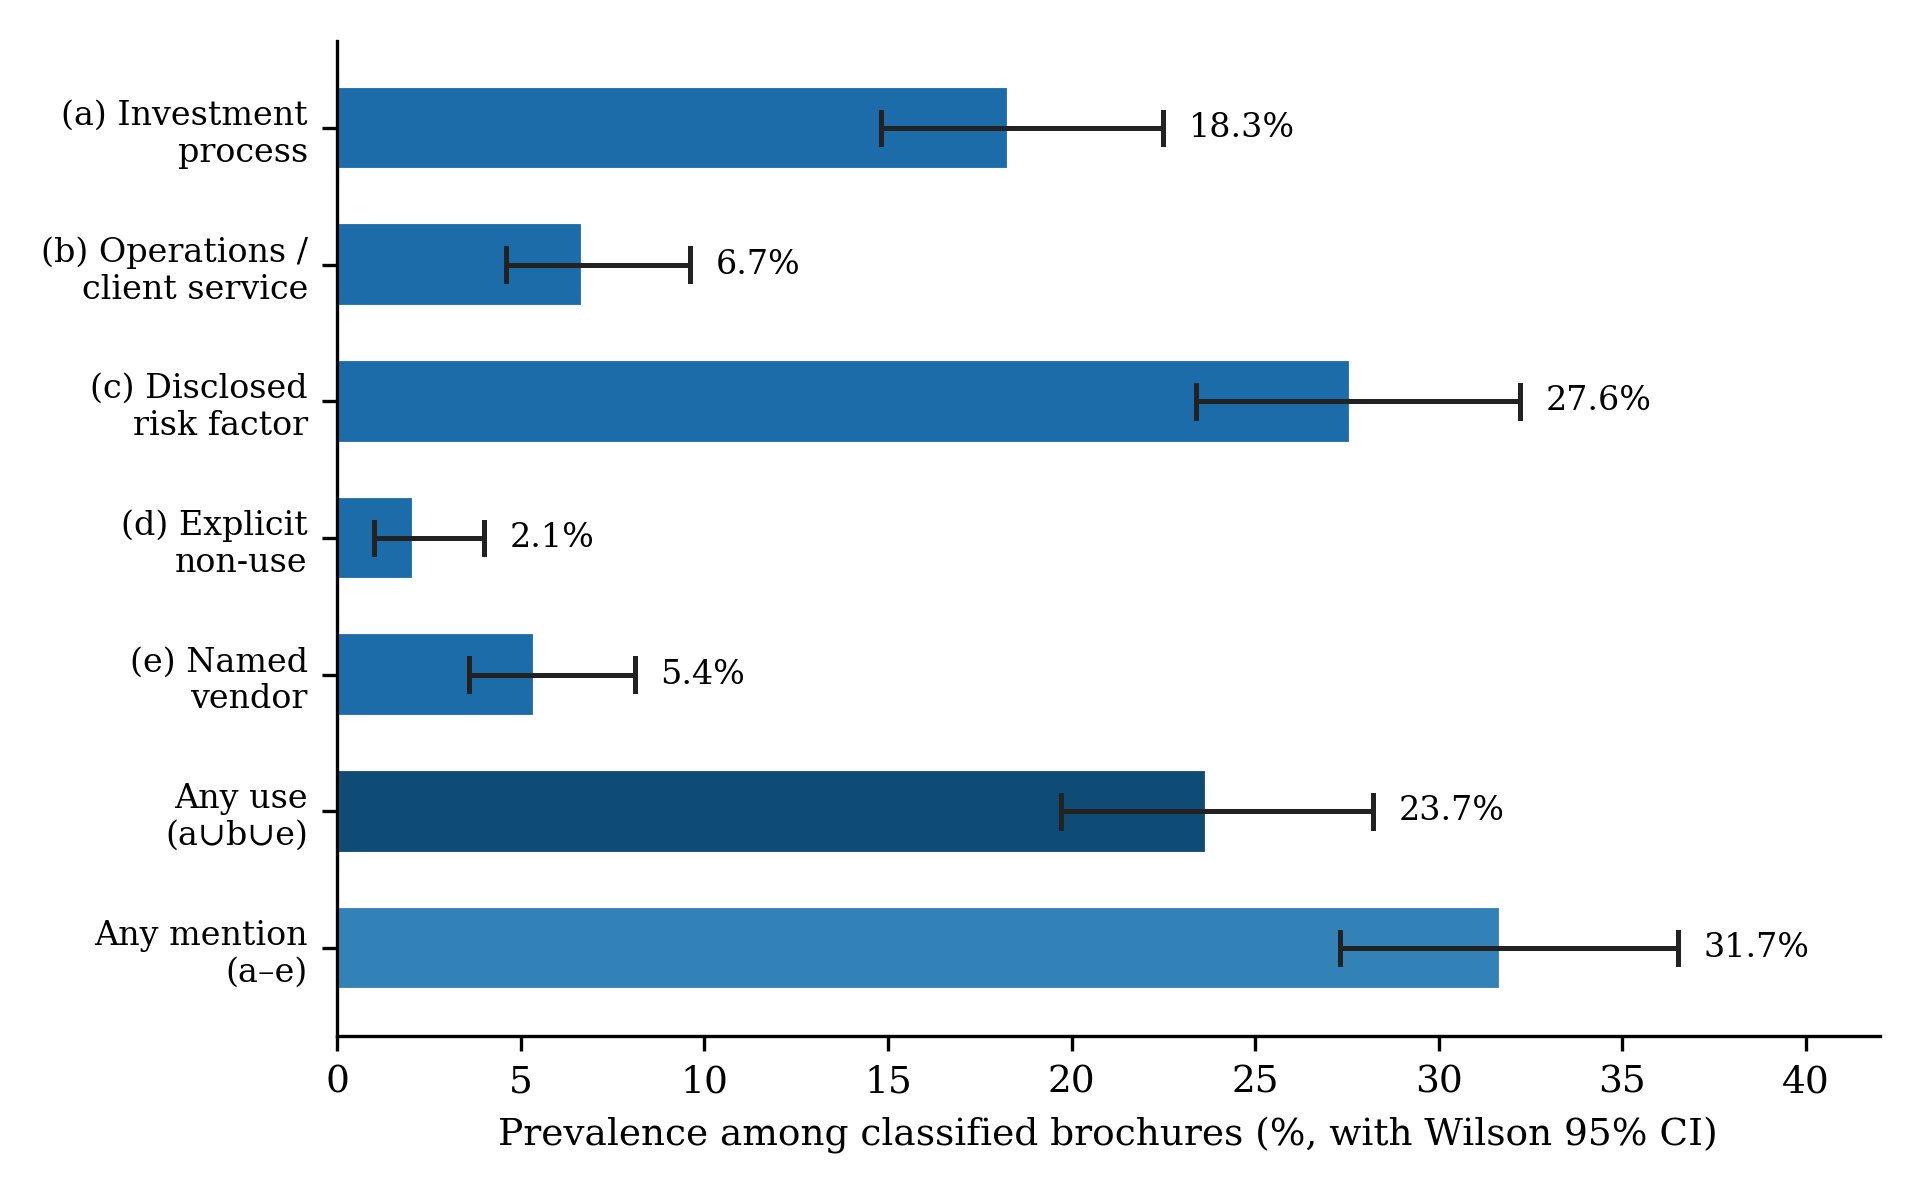
\includegraphics[width=12cm]{figures/fig1}\end{center}
\caption{Prevalence of each typology label among the 388 classified brochures, with Wilson 95\% confidence intervals. The dominant single label is a risk-factor disclosure (c), not a claim of use; explicit non-use (d) is essentially absent.}\label{fig:typology}
\end{figure}

\begin{figure}[h!]
\begin{center}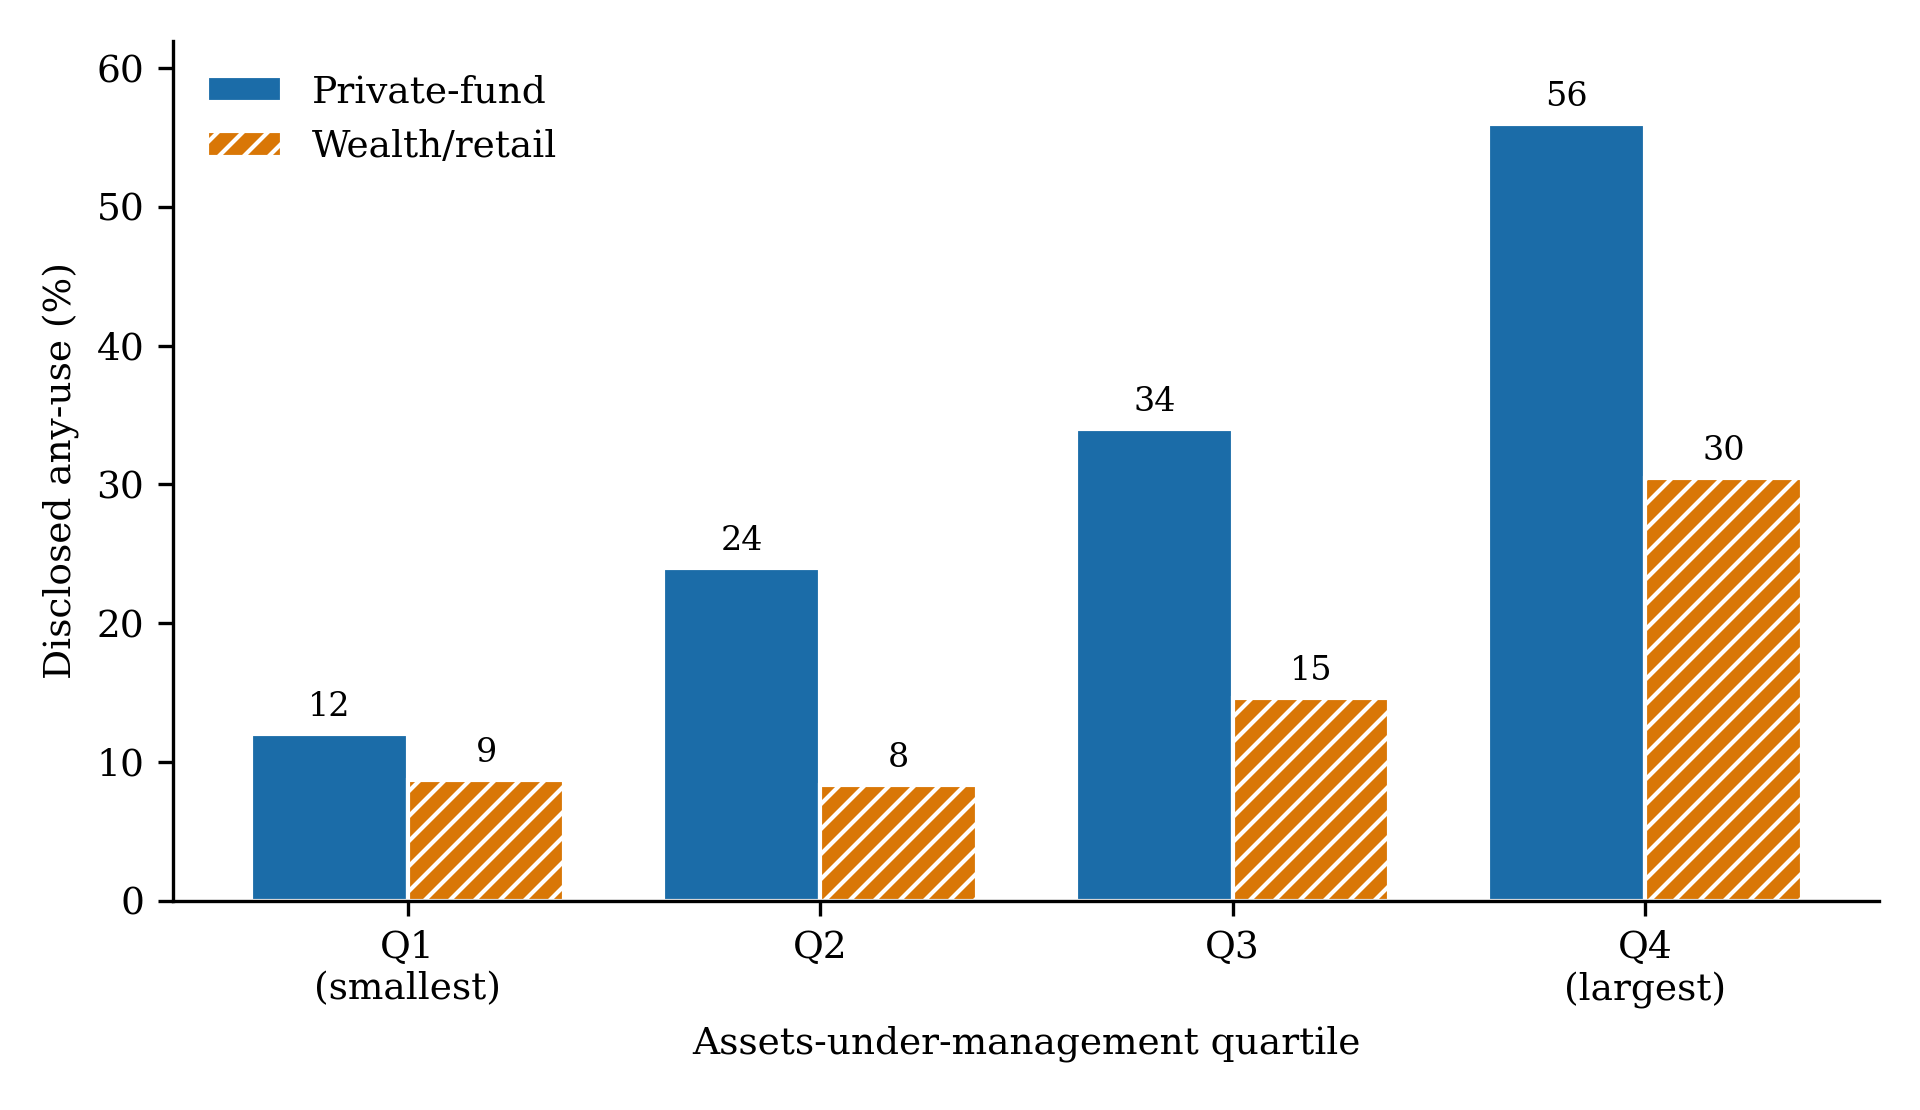
\includegraphics[width=12cm]{figures/fig2}\end{center}
\caption{Disclosed any-use of AI by adviser type and AUM quartile. Bars show the within-stratum share of brochures disclosing any use (labels a, b, or e); private-fund advisers (solid) exceed wealth/retail advisers (hatched) at every size quartile, and disclosure rises strongly with size in both types.}\label{fig:gradient}
\end{figure}

\begin{figure}[h!]
\begin{center}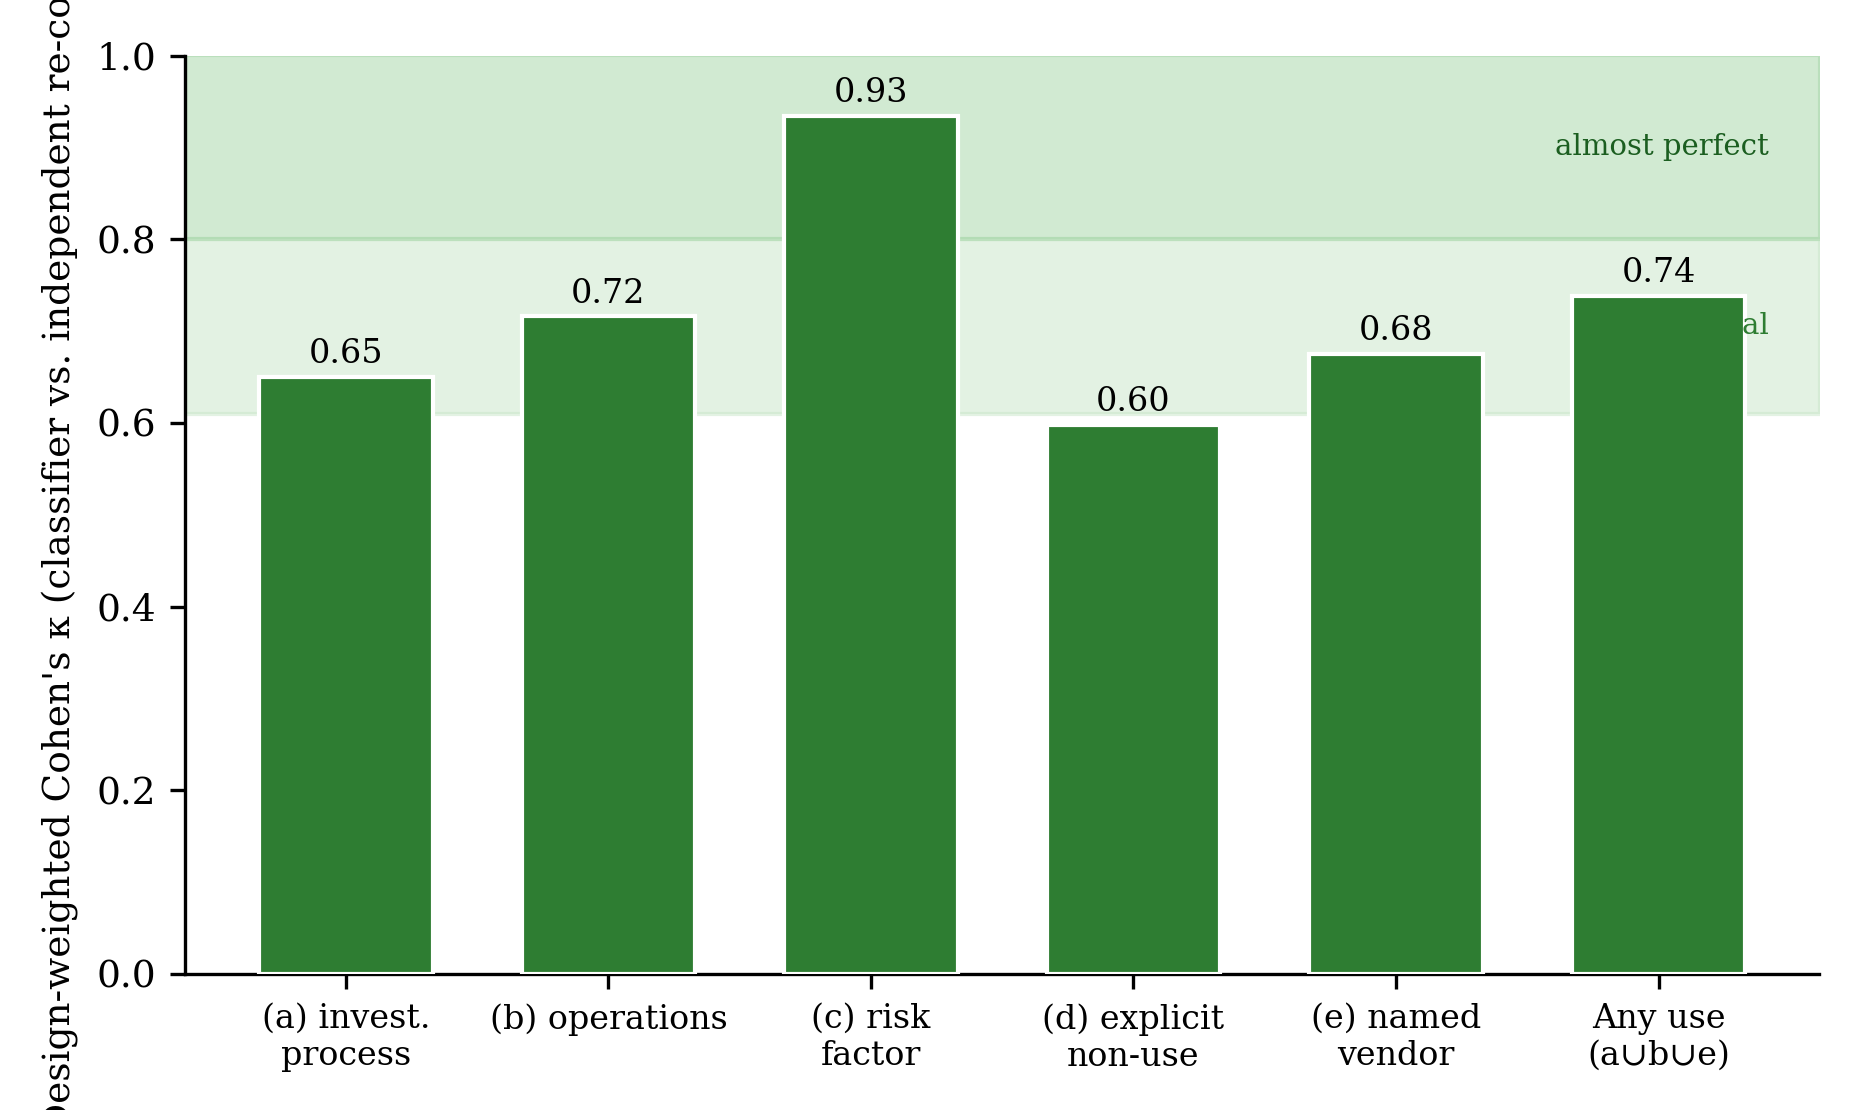
\includegraphics[width=12cm]{figures/fig3}\end{center}
\caption{Independent cross-family validation: design-weighted Cohen's $\kappa$ between the primary classifier (gpt-4o) and a blinded re-coding by a different model family, per label and for the derived any-use indicator (two-phase verification sample, $n = 180$, weighted to the classified population). Shaded bands mark the conventional substantial (0.61--0.80) and almost-perfect ($>0.80$) agreement regions; the risk-factor label is almost-perfect and any-use is comfortably substantial, while the finer investment-process distinction remains the softest construct.}\label{fig:validation}
\end{figure}

\begin{figure}[h!]
\begin{center}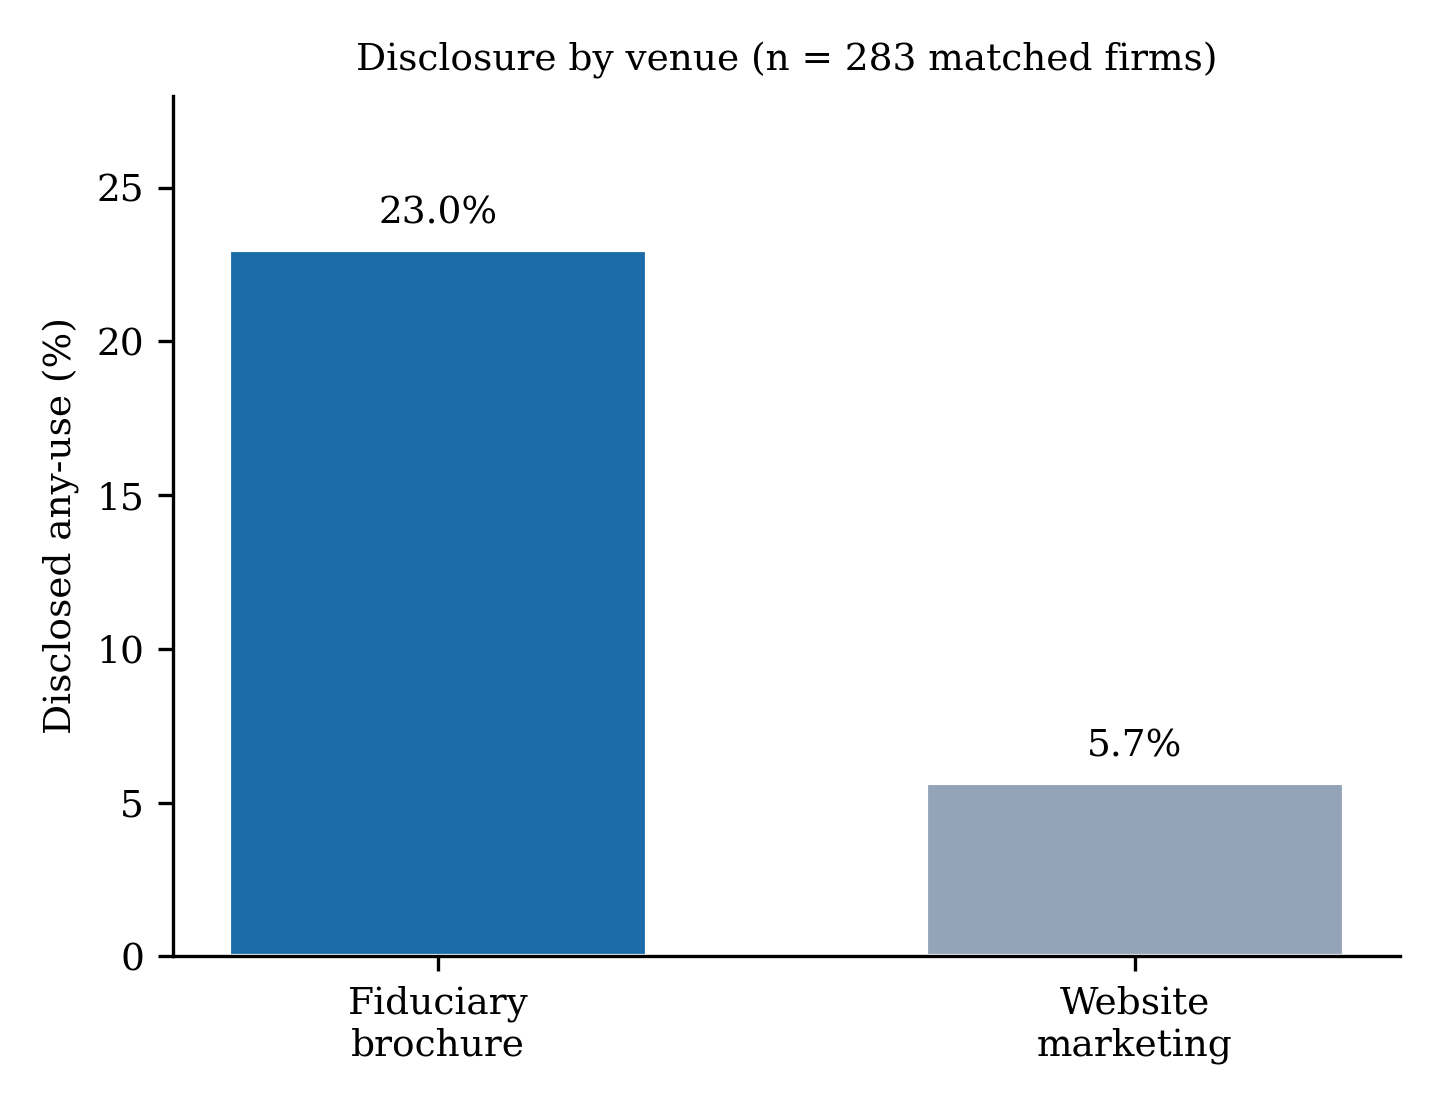
\includegraphics[width=9cm]{figures/fig4}\end{center}
\caption{Disclosed any-use of AI by venue for the 283 firms observed in both venues. Contrary to the intuition motivating AI-washing concern, the fiduciary brochure is the more AI-forward venue: disclosed use is 23.0\% in brochures versus 5.7\% in current website marketing.}\label{fig:venue}
\end{figure}

\end{document}
